\begin{figure}[htbp]
  \centering
  \begin{tabular}{cc}
    \begin{minipage}{0.5\hsize}
      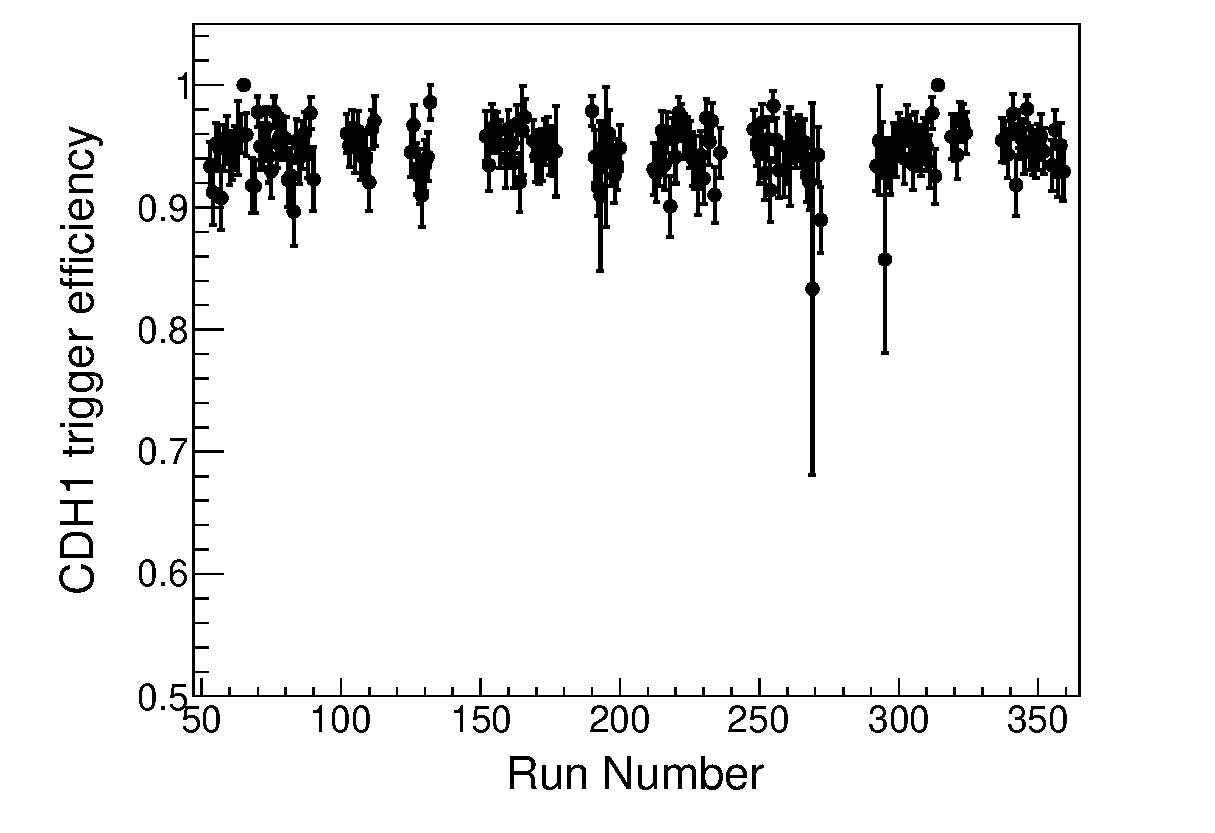
\includegraphics[width=5cm]{../pic/Run68/trigger/CDH1.eps}
    \end{minipage}

    \begin{minipage}{0.5\hsize}
      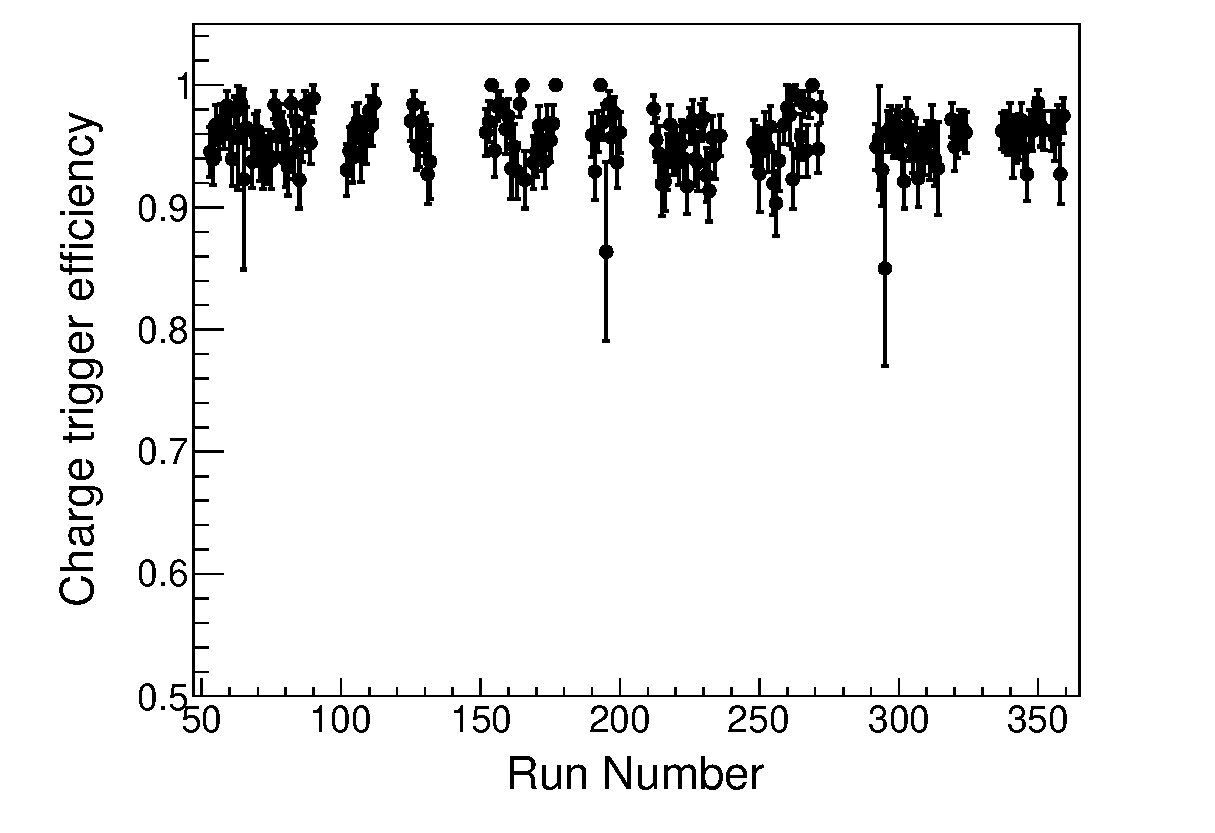
\includegraphics[width=5cm]{../pic/Run68/trigger/Charge.eps}
    \end{minipage}
  \end{tabular}

  \begin{tabular}{cc}
    \begin{minipage}{0.5\hsize}
      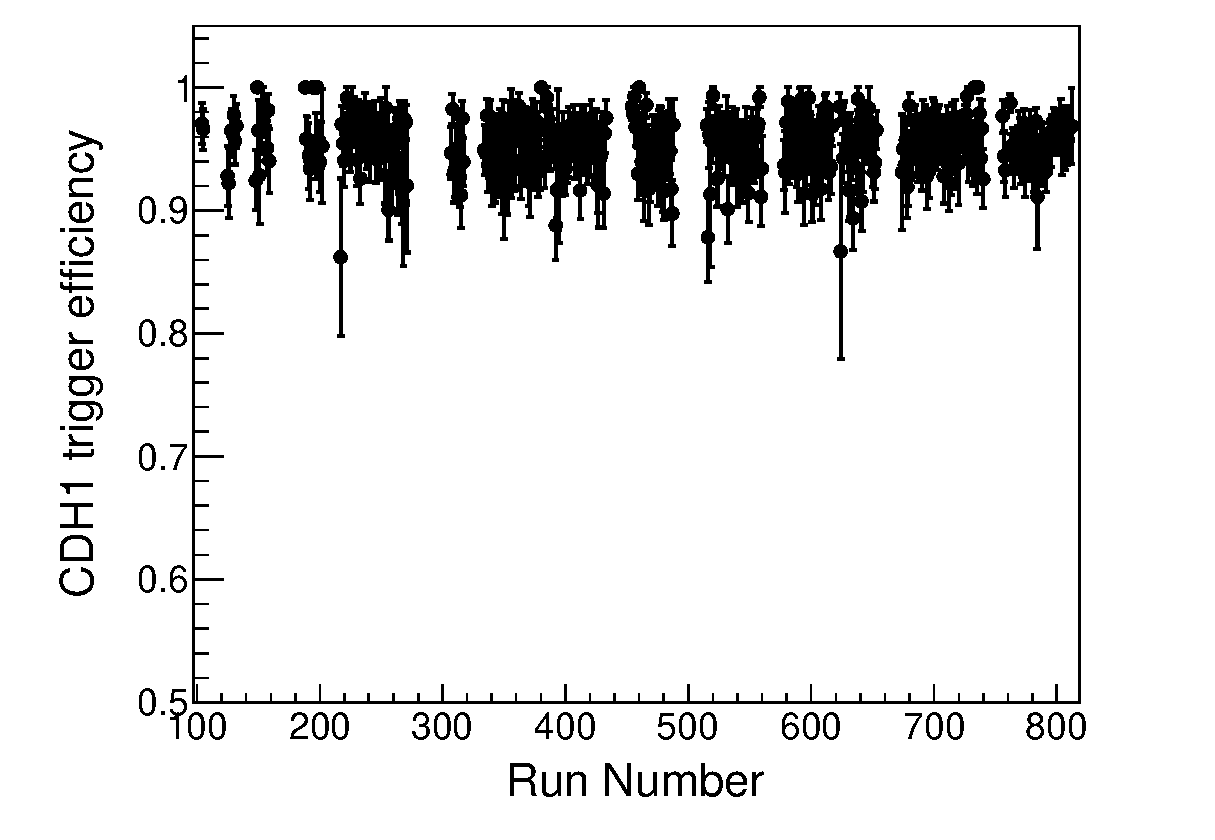
\includegraphics[width=5cm]{../pic/Run78/trigger/CDH1.eps}
    \end{minipage}

    \begin{minipage}{0.5\hsize}
      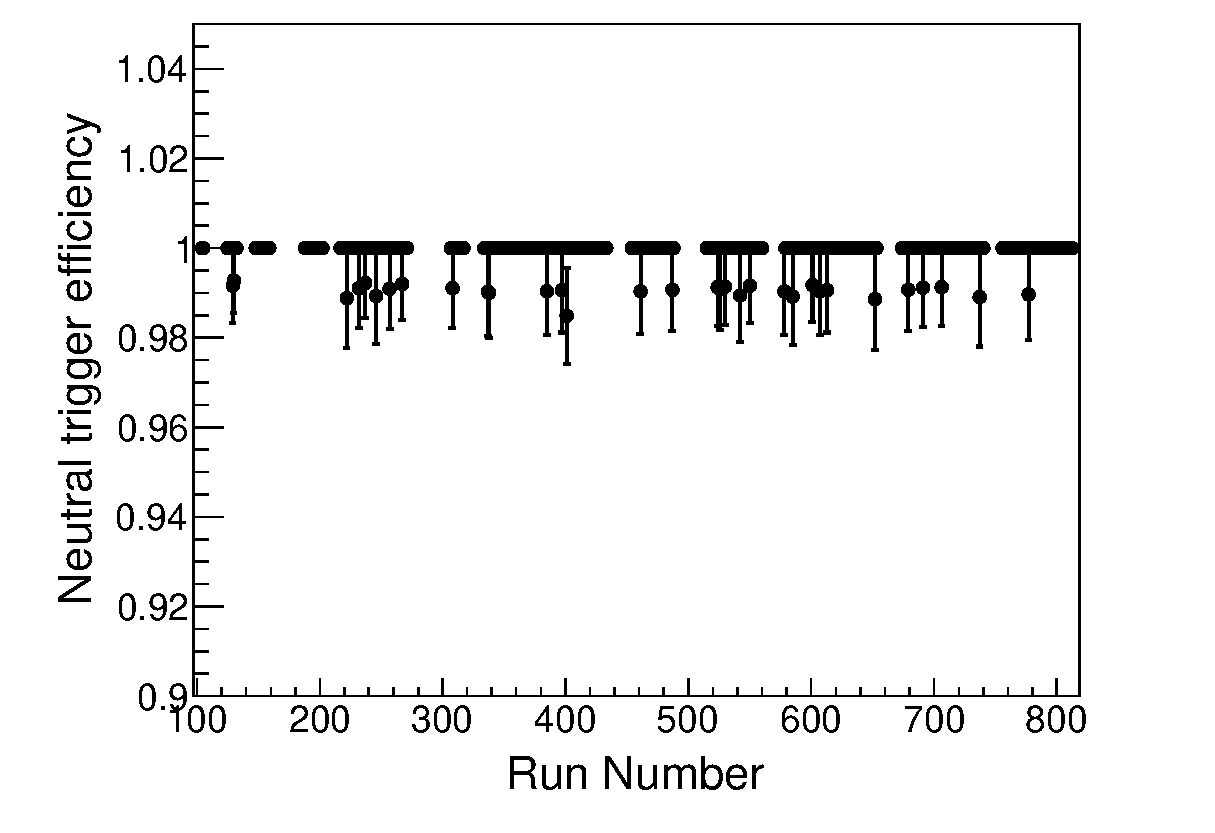
\includegraphics[width=5cm]{../pic/Run78/trigger/Neutral.eps}
    \end{minipage}
  \end{tabular}
  \caption{
    These figures show about trigger efficiencies in each run.
    The $d(K^-, p)$ analysis was analyzed using MR-RUN68 data which is shown in the above.
    The right above shows the K $\otimes$ CDH1 trigger and the left above shows the charge trigger.
    The $d(K^-, n)$ analysis was analyzed using MR-RUN78 data which is shown in the down.
    The right down shows the K $\otimes$ CDH1 trigger and the left down shows the neutral trigger.
  }
  \label{fig:trigger_eff}
\end{figure}
